\documentclass{article}
\usepackage[utf8]{inputenc}
\usepackage{amsmath}
\usepackage{geometry}
\geometry{
 a4paper,
 total={182mm,257mm},
 left=14mm,
 top=20mm,
 }
 \usepackage{amsthm}
 \usepackage[utf8]{inputenc}
 \usepackage[italian]{babel}
\usepackage[T1]{fontenc}
\usepackage{amssymb}
\usepackage{physics}
\usepackage{commath}
\usepackage{tikz}
\usepackage{pgfplots}
\usepackage{graphicx}
\graphicspath{ {Immagini/} }
\usepackage{float}
\usepackage{hyperref}
\hypersetup{
    colorlinks=true,
    linkcolor=red,
    citecolor=green
    filecolor=magenta,      
    urlcolor=cyan,
}


%Theorem Environments
\newtheorem{thm}{Teorema}[section]
\newtheorem{lem}[thm]{Lemma}
\newtheorem{property}{Proprietà}[section]
\newtheorem{defn}{Definizione}[section]
\newtheorem{prop}[defn]{Proposizione}
\newtheorem{example}{Esempi}[subsection]
\newtheorem{exerc}[example]{Esercizi Svolti}

%Commandi di Formattazione
\newcommand{\noi}{\noindent}
\newcommand{\note}{\noindent {\quad \bf \underline{Osservazione:}} \quad}
\newcommand{\eg}{\noindent {\bf \underline{Esempio:}} \quad}
\newcommand{\bfemph}[1]{\textbf{\textit{#1}}}
\renewcommand{\emph}[1]{\bfemph{#1}}

%Number Sets
\newcommand{\R}{\mathbb{R}}
\newcommand{\C}{\mathbb{C}}
\newcommand{\Z}{\mathbb{Z}}
\newcommand{\Q}{\mathbb{Q}}

%Shortcuts
\newcommand{\then}{\ensuremath{\Rightarrow}}
\newcommand{\twopartdef}[4]
{
	\left\{
		\begin{array}{ll}
			#1 & \mbox{se } #2 \\
			#3 & \mbox{se } #4
		\end{array}
	\right.
}

%Vectors
\renewcommand{\i}{\vu{i}}
\renewcommand{\j}{\vu{j}}
\renewcommand{\k}{\vu{k}}
\renewcommand{\a}{\va{a}}
\renewcommand{\b}{\va{b}}
\renewcommand{\c}{\va{c}}
\renewcommand{\v}{\va{v}}
\renewcommand{\u}{\va{u}}
\newcommand{\s}{\va{s}}
\renewcommand{\t}{\va{t}}
\newcommand{\verst}{\vu{t}}
\newcommand{\versr}{\vu{r}}
\renewcommand{\r}{\va{r}}
\newcommand{\tauvs}{\vu{\tau}}
\newcommand{\tauvt}{\va{\tau}}
\newcommand{\normvs}{\vu{n}}
\newcommand{\N}{\va{N}}
\newcommand{\g}{\va{g}}
\newcommand{\F}{\va{F}}
\newcommand{\f}{\va{f}}
\newcommand{\M}{\va{M}}
\renewcommand{\l}{\va{l}}
\newcommand{\p}{\va{p}}
\renewcommand{\P}{\va{P}}
\renewcommand{\L}{\va{L}}


\renewcommand{\c}{\overline{c}}
\title{Il Secondo Principio della Termodinamica}
\author{Roberto Gargiulo}
\date{Ultimo Aggiornamento: \today}


\begin{document}

\maketitle
\tableofcontents

\section{Gli Enunciati}
\begin{defn}[Sorgente]
Un sistema che mantiene la propria temperatura costante.
\end{defn}
\begin{defn}[Enunciato di Clausius]
Non è possibile effettuare una trasformazione termodinamica il cui unico risultato sia il trasferimento di una quantità finita di calore da una sorgente fredda ad una calda.
\end{defn}
\begin{defn}[Enunciato di Kelvin-Planck]
Non è possibile realizzare una trasformazione termodinamica che abbia come unico risultato la trasformazione in lavoro del calore fornito da una sorgente.
\end{defn}
\begin{defn}[Rendimento]
Il rendimento di una macchina termica si definisce come:
\[\eta=\frac{L}{Q_A}=1+\frac{Q_B}{Q_A}\]
\end{defn}
\note L'enunciato di Kelvin equivale a dire che il rendimento di una macchina termica è minore di 1.\\
Dimostriamo ora l'equivalenza di questi due enunciati.
\begin{thm}[Clausius Implica Kelvin]
Supponiamo per assurdo che l'enunciato di Kelvin sia falso. Possiamo quindi costruire una macchina termica K che converte interamente lavoro in calore (ad esempio il Mulinello di Joule). Introduciamo poi un'altra macchina frigorifera $M_f$ su cui la prima macchina compie lavoro in modo che assorba calore dalla prima sorgente e ceda calore ad un'altra sorgente, più calda. L'effetto totale è quindi che la sorgente a temperatura fredda ha ceduto calore ad una sorgente a temperatura più alta. Ciò implica che l'enunciato di Clausius sia falso, abbiamo quindi raggiunto l'assurdo.
\begin{figure}[H]
    \centering
    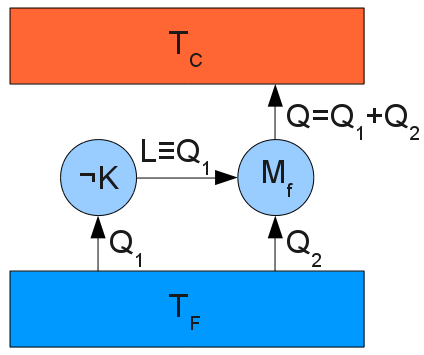
\includegraphics[width=0.5\textwidth]{Kelvin_dimostrazione_assurdo.png}
    \caption{Schema del Sistema Costruito}
    \label{ClausiusKelvin}
\end{figure}
\end{thm}
\begin{thm}[Kelvin Implica Clausius]
Supponiamo per assurdo che l'enunciato di Clausius sia falso. Costruiamo quindi una macchina termica C che assorbe una quantità di calore Q da una sorgente fredda e lo cede ad una calda (in quanto Clausius è falso) come unico risultato. Introduciamo quindi una macchina termica $M_t$ che assorbe una quantità di calore Q' compiendo lavoro L in modo che la quantità di calore ceduta alla sorgente a temperatura minore sia la stessa di quella assorbita dalla macchina C. Abbiamo quindi costruito una trasformazione il cui unico risultato sia quello di convertire calore in lavoro (l'effetto totale è di non coinvolgere la sorgente a temperatura fredda), quindi l'enunciato di Kelvin è falso. Abbiamo raggiunto l'assurdo, come volevasi dimostrare. 
\begin{figure}[H]
    \centering
    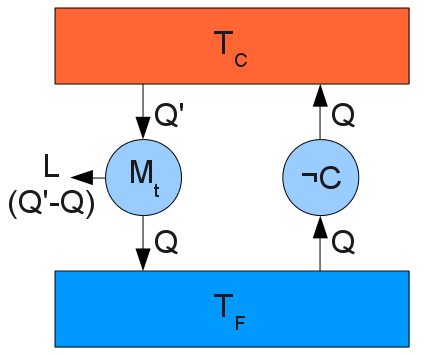
\includegraphics[width=0.5\textwidth]{Clausius_dimostrazione_assurdo.png}
    \caption{Schema del Sistema Costruito}
    \label{KelvinClausius}
\end{figure}
\end{thm}

\section{Teorema di Carnot}
\begin{thm}[Teorema di Carnot]
Ogni macchina reversibile che lavoro tra due sorgenti alla stessa temperatura ha lo stesso rendimento. Qualsiasi altra macchina che lavori tra queste sorgenti ha rendimento non maggiore. Il risultato è indipendente dalle trasformazioni del ciclo. 
\end{thm}
\begin{proof}
Costruiamo due macchine termiche X ed R che lavorano tra le stesse sorgenti e tali da compiere lo stesso lavoro L, assorbendo rispettivamente una quantità di calore $Q_1$ e $Q_1'$ e cedendo una quantità di calore $Q_2$ e $Q_2'$ alla sorgente calda e fredda rispettivamente. 
\begin{figure}[H]
    \centering
    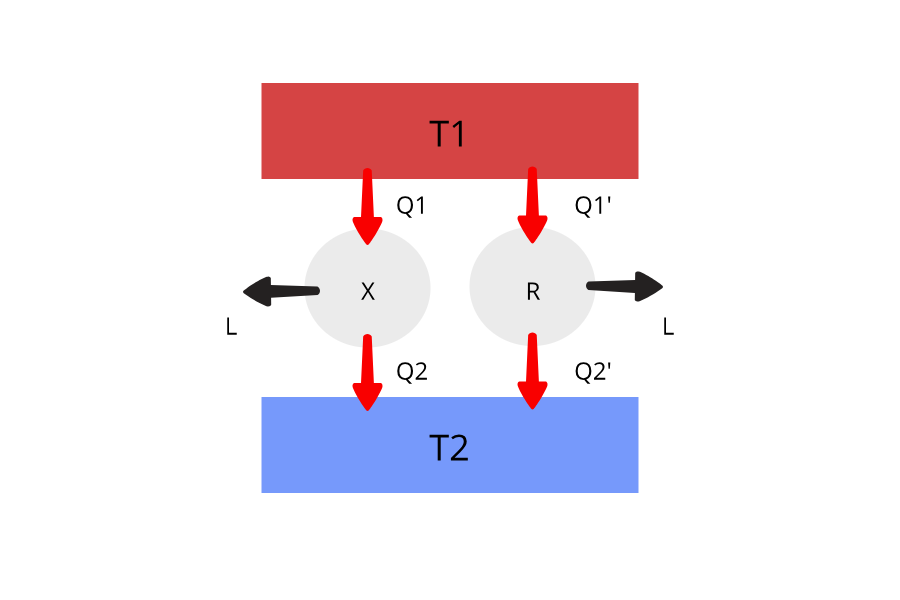
\includegraphics[width=0.7\textwidth]{TeoremaCarnot1.png}
    \label{TeoremaCarnot1}
\end{figure}
Supponendo che la macchina \textbf{R} sia reversibile, utilizziamo il lavoro della macchina \textbf{X} per invertire il ciclo della macchina R in modo che diventi refrigerante (stavolta i calore scambiati da R sono invertiti di segno).
\begin{figure}[H]
    \centering
    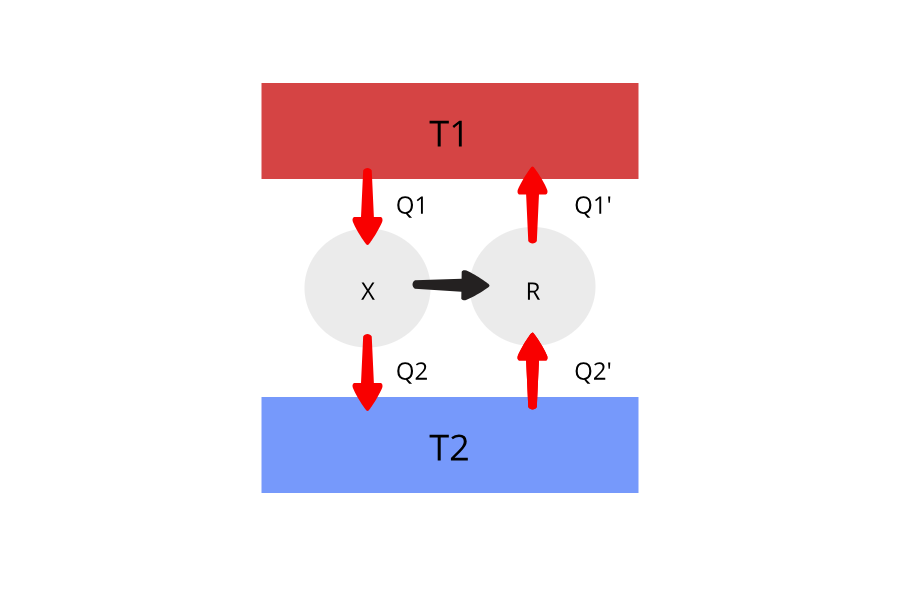
\includegraphics[width=0.7\textwidth]{TeoremaCarnot2.png}
    \label{TeoremaCarnot2}
\end{figure}

Per l'enunciato di Clausius deve risultare che la quantità di calore totale ceduta dalla sorgente calda è maggiore di quella ceduta da quella fredda, quindi otteniamo:
\[\abs{Q_1}\geq\abs{Q_1'}\then \frac{Q_1'}{Q_1}\leq 1\]
Calcoliamo quindi i rendimenti delle due macchine:
\begin{equation}
\eta_X=\frac{L}{Q_1}\quad\eta_R=\frac{L}{Q_1'}\then \eta_X\abs{Q_1}=\eta_R\abs{Q_1'}\then \eta_X=\eta_R\frac{\abs{
Q_1'}}{\abs{Q_1}} \leq \eta_R\then\boxed{\eta_X\leq\eta_R}
\end{equation}

Abbiamo dimostrato la \textbf{prima parte della tesi}. Dimostriamo ora la seconda.
Supponiamo che X sia reversibile, allora possiamo invertire i ragionamenti fatti in modo da ottenere:
\[\eta_X\geq\eta_R\]
Ma allora l'unica possibilità è che i due rendimenti coincidano:
\begin{equation}
\boxed{\eta_X=\eta_R}
\end{equation}
\end{proof}
\note Il risultato è indipendente dalle trasformazioni del ciclo in quanto l'unica proprietà che abbiamo assunto dalle macchine è che una fosse reversibile.\\
\note L'uguaglianza come caso limite nel primo risultato è nel caso in cui entrambe le macchine siano irreversibili oppure nel caso $Q_1=Q_1'=0\iff L=0$ ossia la macchina sta operando alcuna trasformazione.

\begin{prop}[Definizione di Temperatura Assoluta]
Dimostrato il Teorema di Carnot siamo in grado di dare una definizione assoluta di temperatura utilizzando il risultato per cui ogni macchina reversibile che opera tra certe due sorgenti ha lo stesso rendimento, ciò implica che il rendimento di una macchina reversibile R è funzione delle due temperature:
\[\eta=\eta(t_1,t_2)=1+\frac{Q_2}{Q_1}\]
Definiamo quindi la funzione g come segue:
\[g(t_1,t_2)=1-\eta(t_1,t_2)=\frac{\abs{Q_2}}{\abs{Q_1}}\]
Costruiamo poi il seguente sistema formato da tre sorgenti e due macchine termiche nel modo seguente (dove $\abs{Q_2}=\abs{Q_2'}$):
\begin{figure}[H]
    \centering
    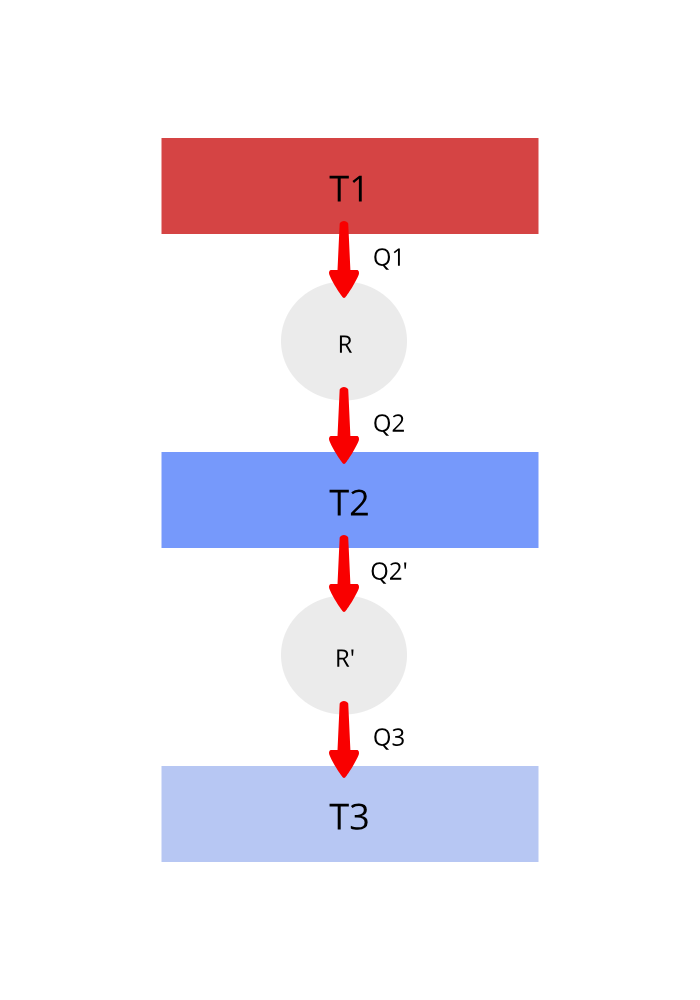
\includegraphics[width=0.4\textwidth]{TemperaturaAssoluta.png}
    \label{TeoremaCarnot2}
\end{figure}
Corto-circuitiamo le due macchine termiche in modo da ottenere un'unica macchina termica reversibile che lavora tra la sorgente a temperatura $t_1$ e quella a temperatura $t_3$ scambiando rispettivamente una quantità di calore $Q_1$ e $Q_3$.
\begin{figure}[H]
    \centering
    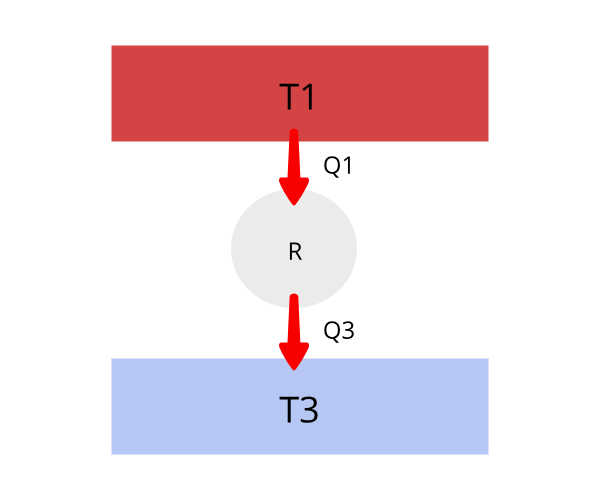
\includegraphics[width=0.5\textwidth]{TempAss.png}
\end{figure}
La funzione g di questa macchina termica è:
\[g(t_1,t_3)=\frac{\abs{Q_3}}{\abs{Q_1}}\]
Mentre delle due macchine singolarmente:
\[g(t_1,t_2)=\frac{\abs{Q_2}}{\abs{Q_1}}\quad g(t_2,t_3)=\frac{\abs{Q_3}}{\abs{Q_2'}}\]
Allora vale la relazione:
\[g(t_1,t_3)=g(t_1,t_2)\cdot g(t_2,t_3)\quad\forall t_2\]
Ciò significa che g è una funzione indipendente da $t_2$. Possiamo scriverla quindi come rapporto di una funzione f applicata in $t_3$ e applicata in $t_2$:
\[g(t_1,t_3)=\frac{f(t_3)}{f(t_1)}\]
Chiamiamo questa funzione f(t) \textbf{temperatura termodinamica assoluta} e poniamo $g(P.T.)=T_{pt}=273,16K$ ossia poniamo la temperatura assoluta del punto triplo (un punto termodinamico ben definito) dell'acqua uguale a $273,16K$. Possiamo quindi misurare la temperatura $T_x$ di una sorgente misurando i calori scambiati con una macchina che lavoro tra $T_{pt}$ e $T_x$:
\[T_x=T_{pt}\frac{\abs{Q_x}}{\abs{Q_{pt}}}\]
Ossia il II Principio fornisce un metodo di misurazione \textbf{assoluta} di temperatura.
\end{prop}
\note La scala assoluta e la scala Kelvin coincidono in quanto:
\[\frac{T_x}{T_{pt}}=\frac{\theta_x}{\theta_{pt}}=\frac{\theta_x}{T_{pt}}\iff T_x=\theta_x\]

\subsection{Il Ciclo di Carnot}
Il Ciclo di Carnot è un ciclo composto da quattro trasformazioni reversibili:
\begin{enumerate}
    \item AB \textbf{Espansione Isoterma} ($Q>0$)
    \item BC \textbf{Espansione Adiabatica} ($Q=0$)
    \item CD \textbf{Compressione Isoterma} ($Q<0$)
    \item DA \textbf{Compressione Adiabatica} ($Q=0$)
\end{enumerate}
\begin{figure}[H]
    \centering
    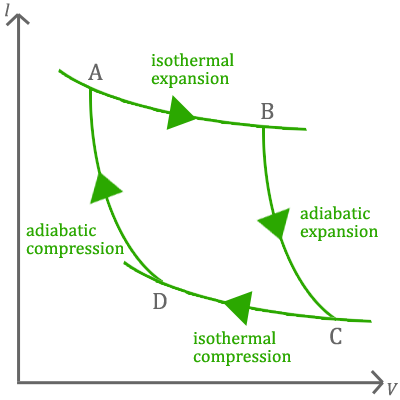
\includegraphics[width=0.6\textwidth]{CicloCarnot.png}
    \caption{Il Ciclo di Carnot}
    \label{CicloCarnot}
\end{figure}
Si può dimostrare che questa è l'unica trasformazione ciclica (percorsa nel senso in figura, tale che la macchina si comporti da macchina termica e \textit{compia} lavoro) che avviene solo tra due sorgenti (e quindi \textbf{due temperature}. Studiamo ora quanto vale il rendimento di una macchina (detta \textbf{macchina di Carnot}) che compie questo ciclo. \\
Durante l'espansione isoterma AB il calore è assorbito dalla sorgente calda a temperatura $T_2$ (uguale al lavoro compiuto dal sistema) e vale:
\[Q_2=nRT_1\ln\frac{V_B}{V_A}\]
Durante l'espansione adiabatica BC vale la relazione tra volume e temperatura:
\[T_BV_B^{\gamma-1}=T_CV_C^{\gamma-1}\iff T_2V_B^{\gamma-1}=T_1V_C^{\gamma-1}\then \left(\frac{V_C}{V_B}\right)^{\gamma-1}=\frac{T_2}{T_1}\]
Durante la compressione isoterma CD il calore ceduto:
\[Q_1=nRT_1\ln\frac{V_D}{V_C}\]
E infine dalla compressione adiabatica DA otteniamo:
\[T_DV_D^{\gamma-1}=T_AV_A^{\gamma-1}\iff T_1V_D^{\gamma-1}=T_2V_A^{\gamma-1}\then \left(\frac{V_D}{V_A}\right)^{\gamma-1}=\frac{T_2}{T_1}\]
Combinando le due equazioni ottenute dalle adiabatiche:
\[\left(\frac{V_C}{V_B}\right)^{\gamma-1}=\frac{T_2}{T_1}=\left(\frac{V_D}{V_A}\right)^{\gamma-1}\then \frac{V_C}{V_B}=\frac{V_D}{V_A}\then\boxed{\frac{V_C}{V_D}=\frac{V_B}{V_A}}\]
Il rendimento del ciclo vale 
\begin{equation}
\begin{split}
    \eta&=1+\frac{Q_1}{Q_2}=1+\frac{nRT_B\ln\frac{V_D}{V_C}}{nRT_A\ln\frac{V_B}{V_A}}=\\
    &=1+\frac{T_1\ln\frac{V_D}{V_C}}{T_2\ln\frac{V_B}{V_A}}=1-\frac{T_1\ln\frac{V_C}{V_D}}{T_2\ln\frac{V_B}{V_A}}=\\
    &=\boxed{1-\frac{T_1}{T_2}}
\end{split}
\end{equation}
Come volevasi dimostrare, il rendimento di una macchina di Carnot dipende unicamente dalle temperature delle \textit{due} sorgenti tra cui opera. Inoltre usando il \textbf{Teorema di Carnot} ricaviamo che una macchina qualunque che opera tra due sorgenti (e quindi compie lo stesso tipo di trasformazioni, anche se irreversibili) ha un rendimento:
\[\eta\leq1-\frac{T_1}{T_2}\]
Inoltre per definizione di rendimento:
\[\eta=1+\frac{Q_1}{Q_2}\then \frac{Q_1}{Q_2}\leq -\frac{T_1}{T_2}\then \boxed{\frac{Q_1}{T_1}+\frac{Q_2}{T_2}}\]
Questa disuguaglianza è particolarmente importante in quanto rappresenta una prima forma di enunciato per il secondo principio della termodinamica, ma deve essere generalizzato in quanto per trovare questo risultato abbia supposto due ipotesi:
\begin{enumerate}
    \item La trasformazione operata dalla macchina è \textbf{ciclica}
    \item La macchina termica opera tra \textbf{due sorgenti}
\end{enumerate}

\section{L'Entropia}
\begin{thm}[Teorema di Clausius]
Il Teorema di Clausius permette di generalizzare il risultato ottenuto ad un numero arbitrario di sorgenti (fino ad una continuità di sorgenti). Consideriamo prima di tutto una macchina termica che compie una trasformazione ciclica tra n sorgenti:
\begin{figure}[H]
    \centering
    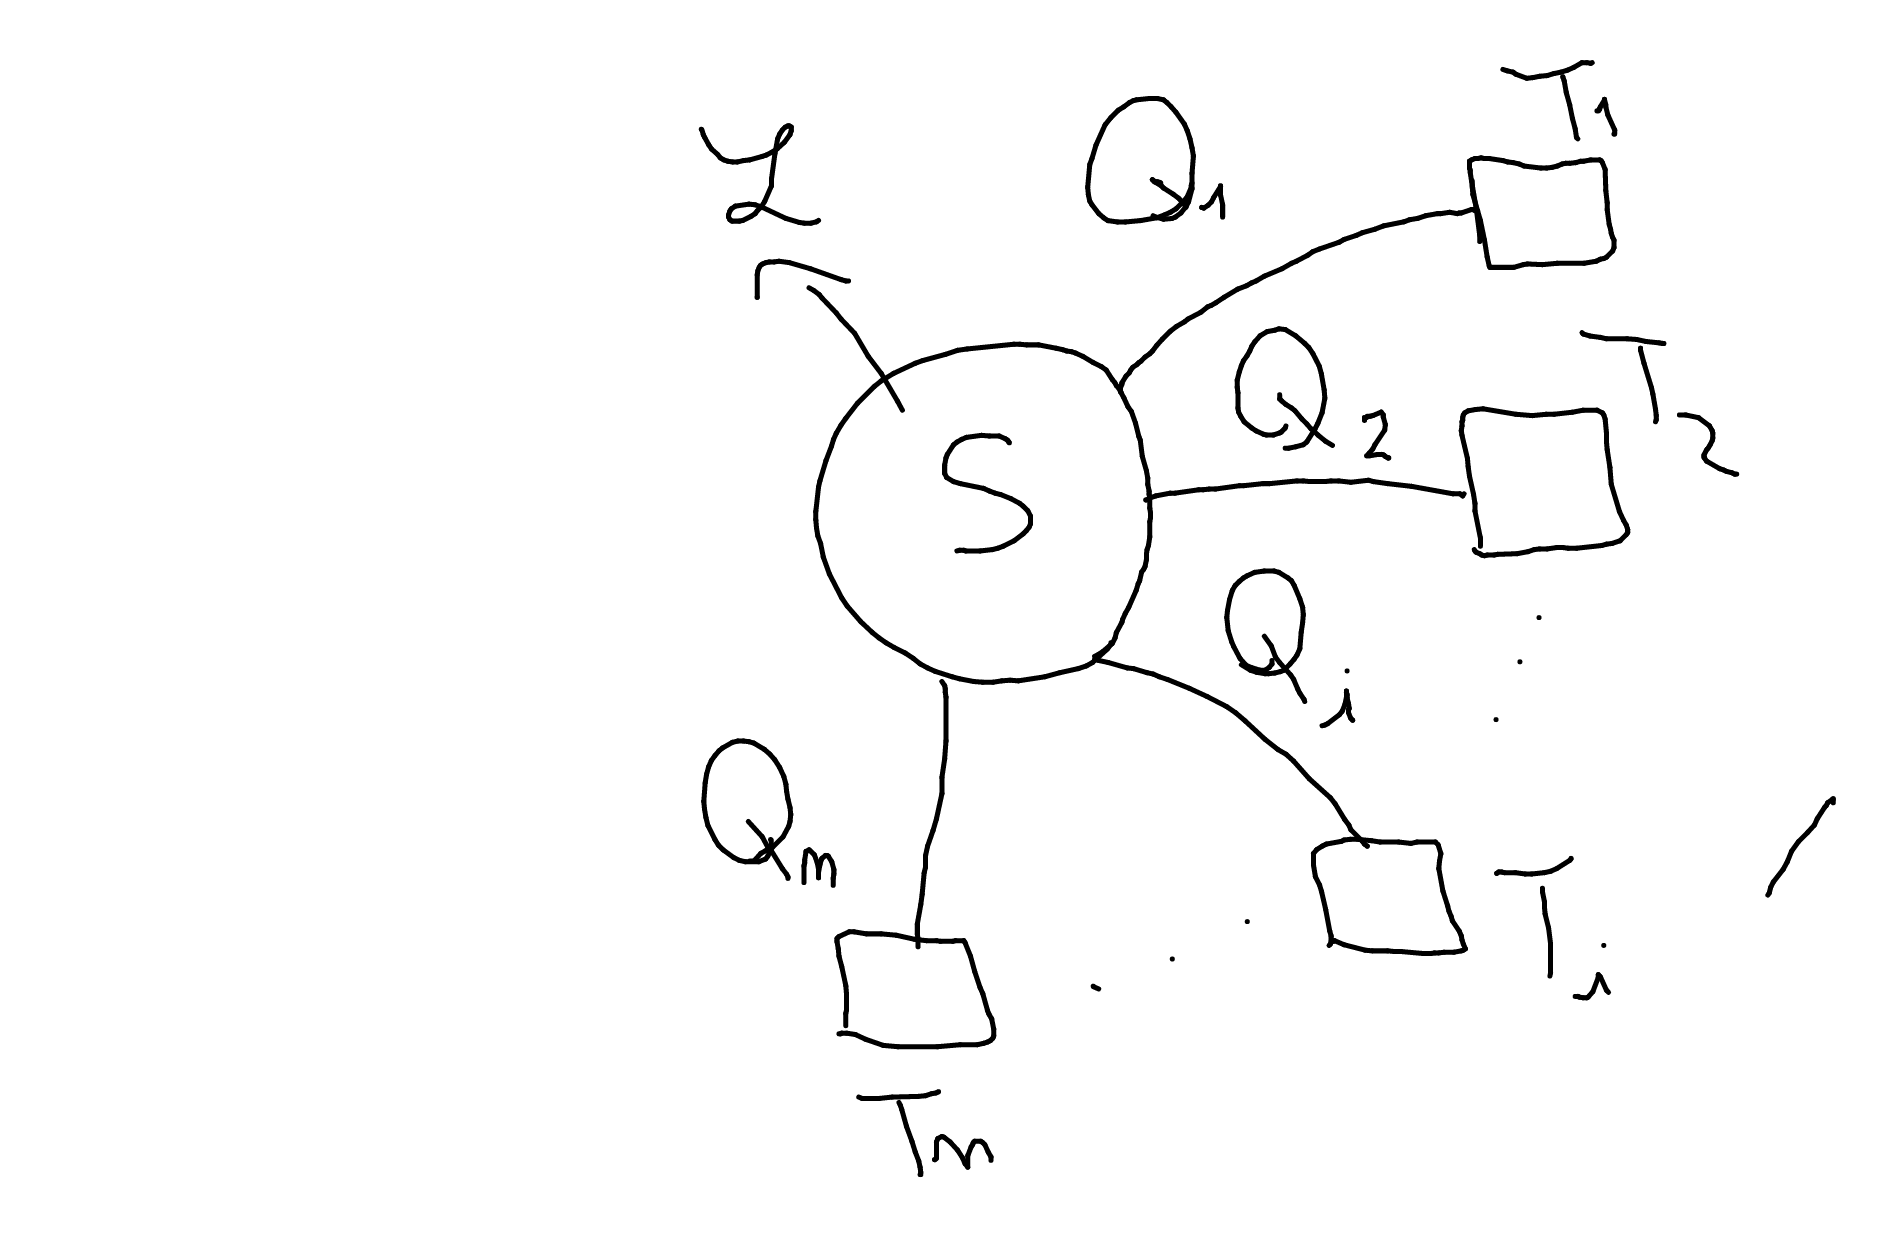
\includegraphics[width=0.5\textwidth]{TeoremaClausius1.png}
    \label{TeoremaClausius1}
\end{figure}
Introduciamo poi n macchine di Carnot reversibili che lavorano tra una sorgente a temperatura $T_0$ e l'i-esima sorgente a temperatura $T_i$, scambiando rispetivamente un certo calore $Q_{i0}$ con la prima sorgente e $-Q_i$ con le altre:
\begin{figure}[H]
    \centering
    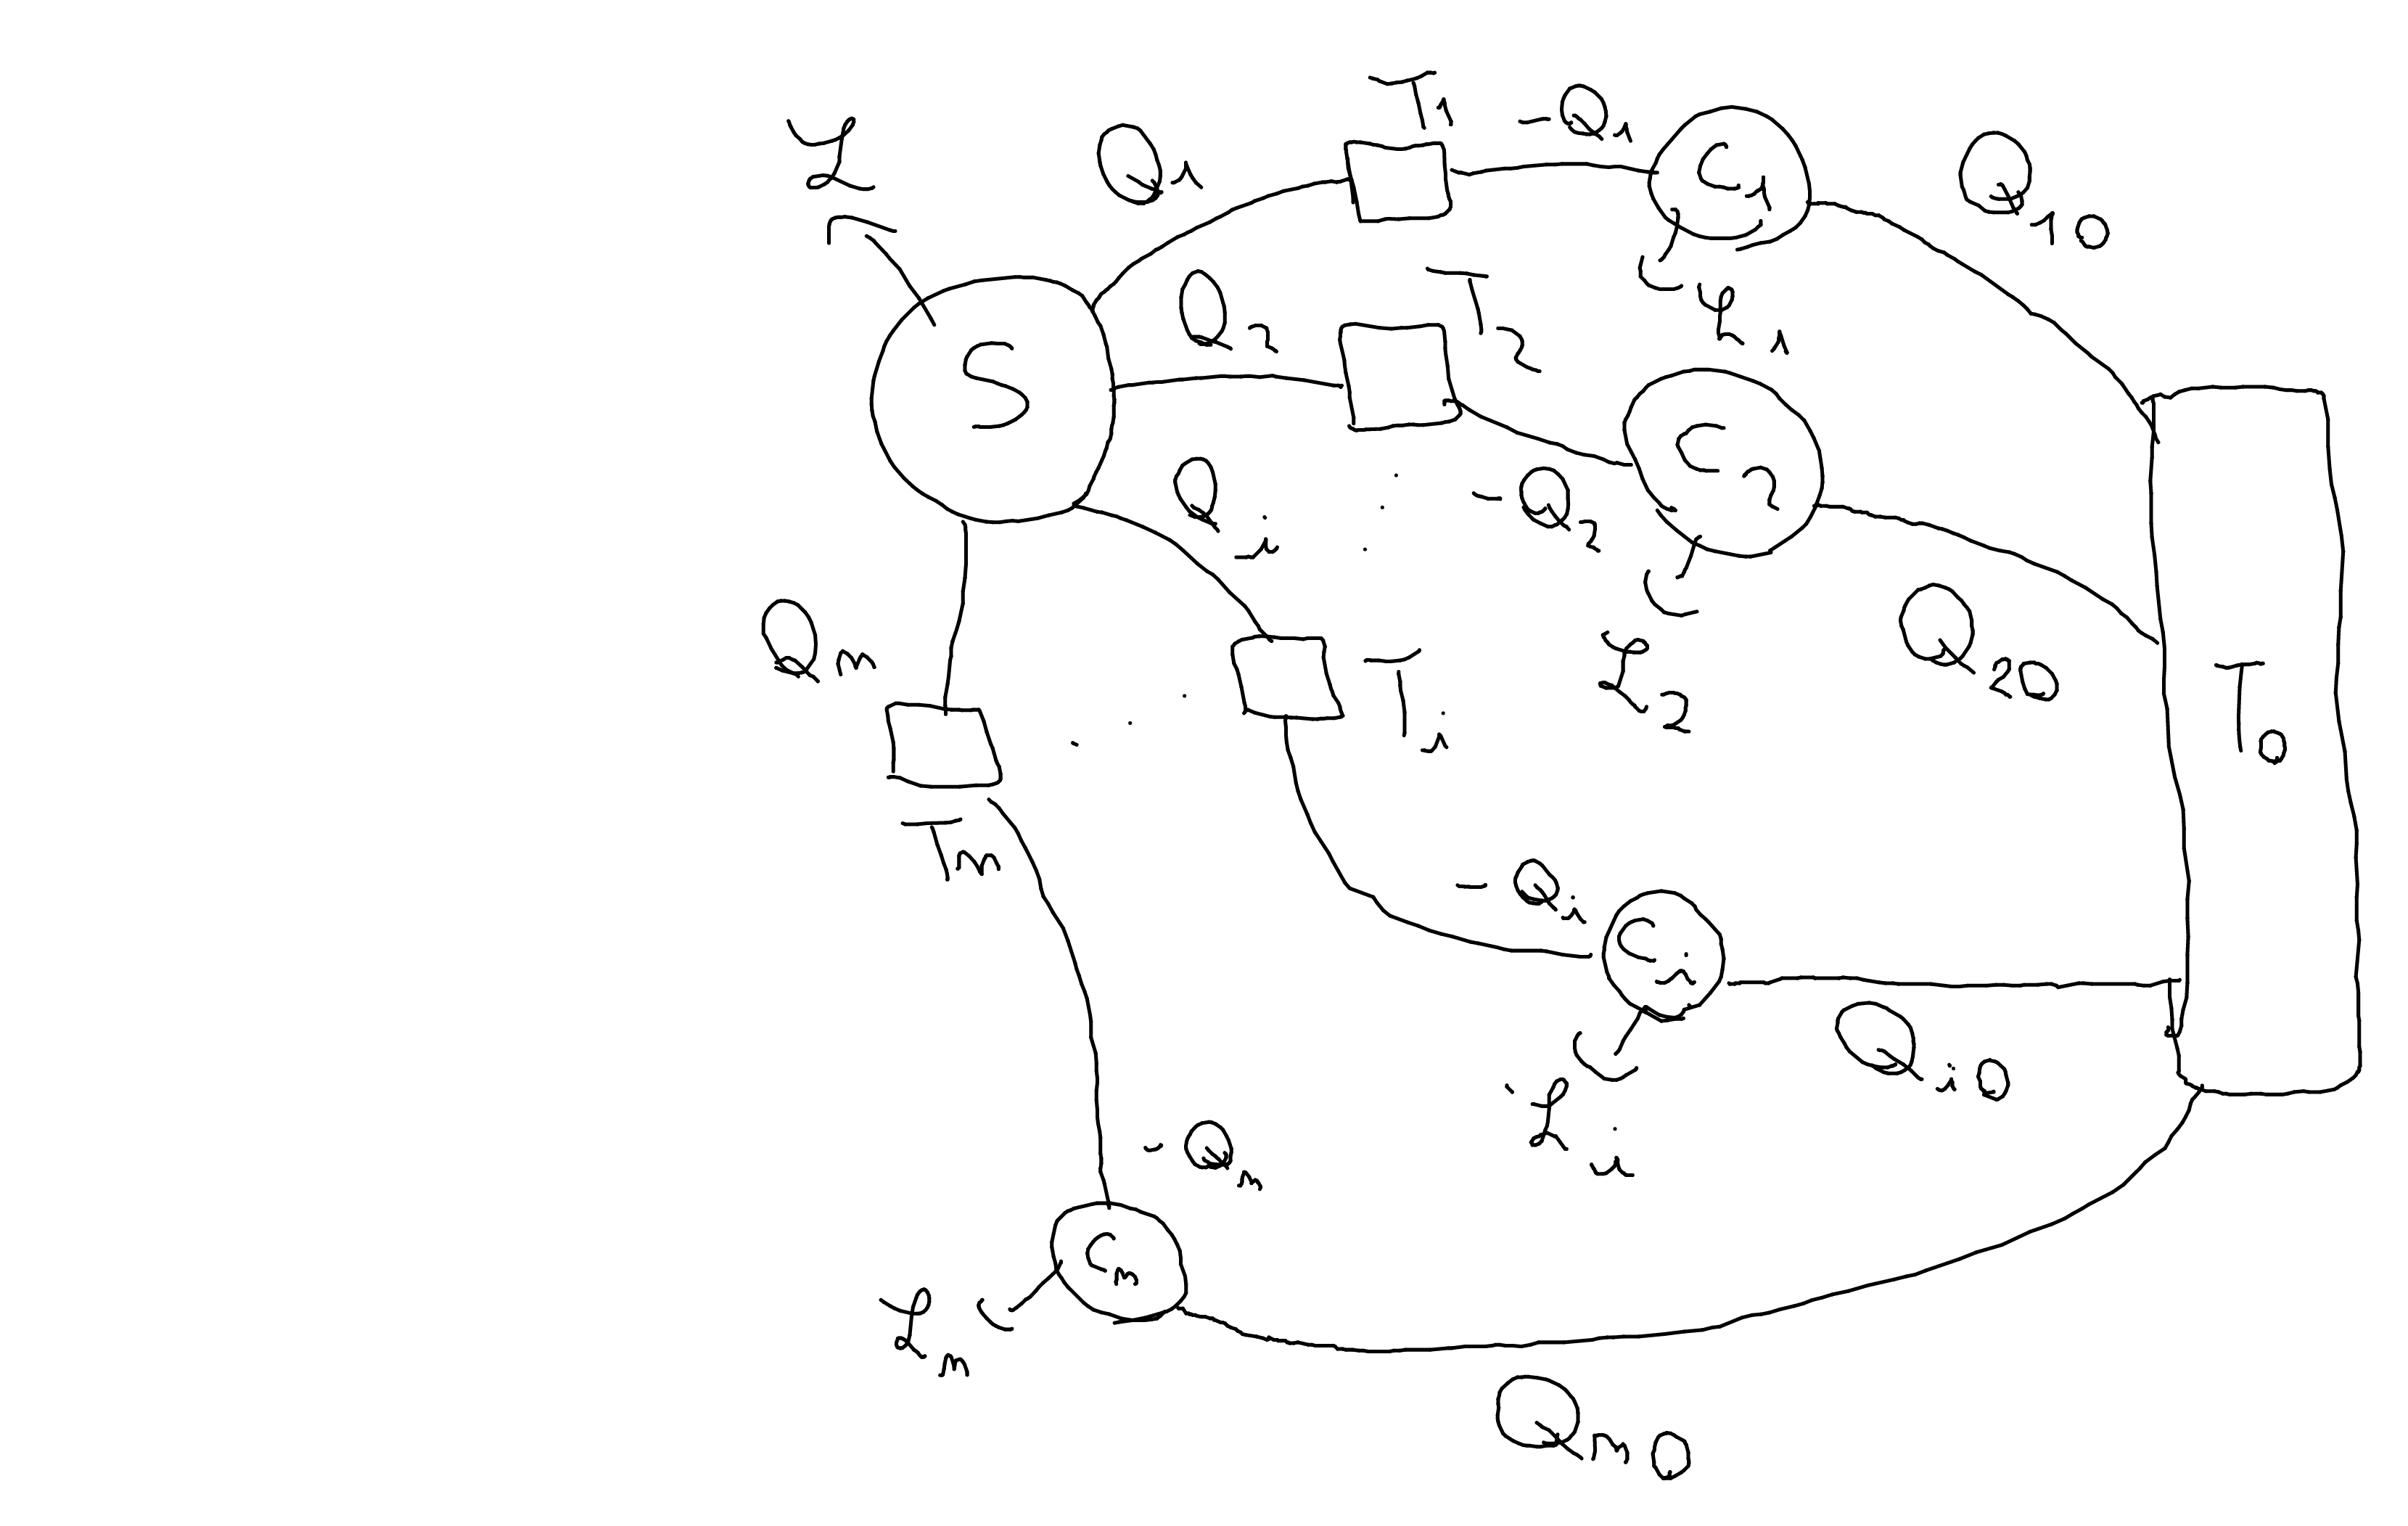
\includegraphics[width=0.5\textwidth]{TeoremaClausius2.png}
    \label{TeoremaClausius2}
\end{figure}
Abbiamo quindi effettivamente circuitato le sorgenti, ossia abbiamo costruito una nuova macchina termica che compie una trasformazione ciclica. Il calore totale scambiato dalla sorgente a temperatura $T_0$ deve essere tuttavia \textbf{ceduto} (o nullo) per l'enunciato di Kelvin (in quanto se fosse positivo l'unico risultato della trasformazione ciclica sarebbe il lavoro del sistema). Inoltre per il Teorema di Carnot applicato a ciascuna delle macchine termiche $C_i$ otteniamo:
\[-\frac{Q_i}{T_i}+\frac{Q_{i0}}{T_0}=0\then \frac{Q_{i0}}{T_0}=\frac{Q_i}{T_i}\]
Sommando sull'indice i otteniamo (detto $Q_0$ il calore totale ceduto dalla sorgente a temperatura $T_0$):
\[\sum_i\frac{Q_i}{T_i}=\sum_i\frac{Q_{i0}}{T_0}=\frac{Q_0}{T_0}\leq0\then \boxed{\frac{Q_i}{T_i}\leq0}\]
Questa relazione è nota come \textbf{disuguaglianza di Clausius}. Nel caso particolare in cui la macchina termia S compia una trasformazione ciclica reversibile otteniamo:
\begin{equation}
\boxed{\sum_i\frac{Q_i}{T_i}=0}
\end{equation}
Per un numero arbitrariamente grande di sorgenti (e quindi macchine di Carnot) otteniamo invece l'\textbf{integrale di Clausius} per una macchina reversibile:
\begin{equation}
    \boxed{\oint\frac{\delta Q}{T_{sorgente}}=\oint\frac{\delta Q}{T}=0}
\end{equation}
Che consiste nell'approssimare un qualunque ciclo con dei cicli di Carnot:
\begin{figure}[H]
    \centering
    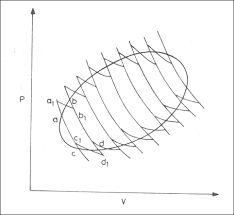
\includegraphics[width=0.3\textwidth]{IntegraleClausius.png}
    \caption{Approssimazione di un qualunque Ciclo Reversibile con dei Cicli di Carnot}
    \label{IntegraleClausius}
\end{figure}
In generale vale la disuguaglianza:
\begin{equation}
\boxed{\oint\frac{\delta Q}{T}\leq0}
\end{equation}
\end{thm}
\begin{prop}[Generalizzazione ad una Trasformazione Aperta]
Dal teorema di Clausius ricaviamo l'importante risultato che è l'integrale o la somma di Clausius, entrambe uguali a 0 per macchine reversibili:
\[\oint\frac{\delta Q}{T}=0\quad\sum_i\frac{Q_i}{T_i}=0\]
Dall'integrale di Clausius si può dimostrare che esiste una funzione di stato S tale che:
\begin{equation}
\boxed{\dif S=\frac{\delta Q}{T}}
\end{equation}
Questa funzione di stato prende il nome di \textbf{entropia}.
Consideriamo ora una generica trasformazione AB (schematizzata in figura come irreversibile) e immaginiamo di compiere una trasformazione reversibile BA in modo tale da ottenere un ciclo. 
\begin{figure}[H]
    \centering
    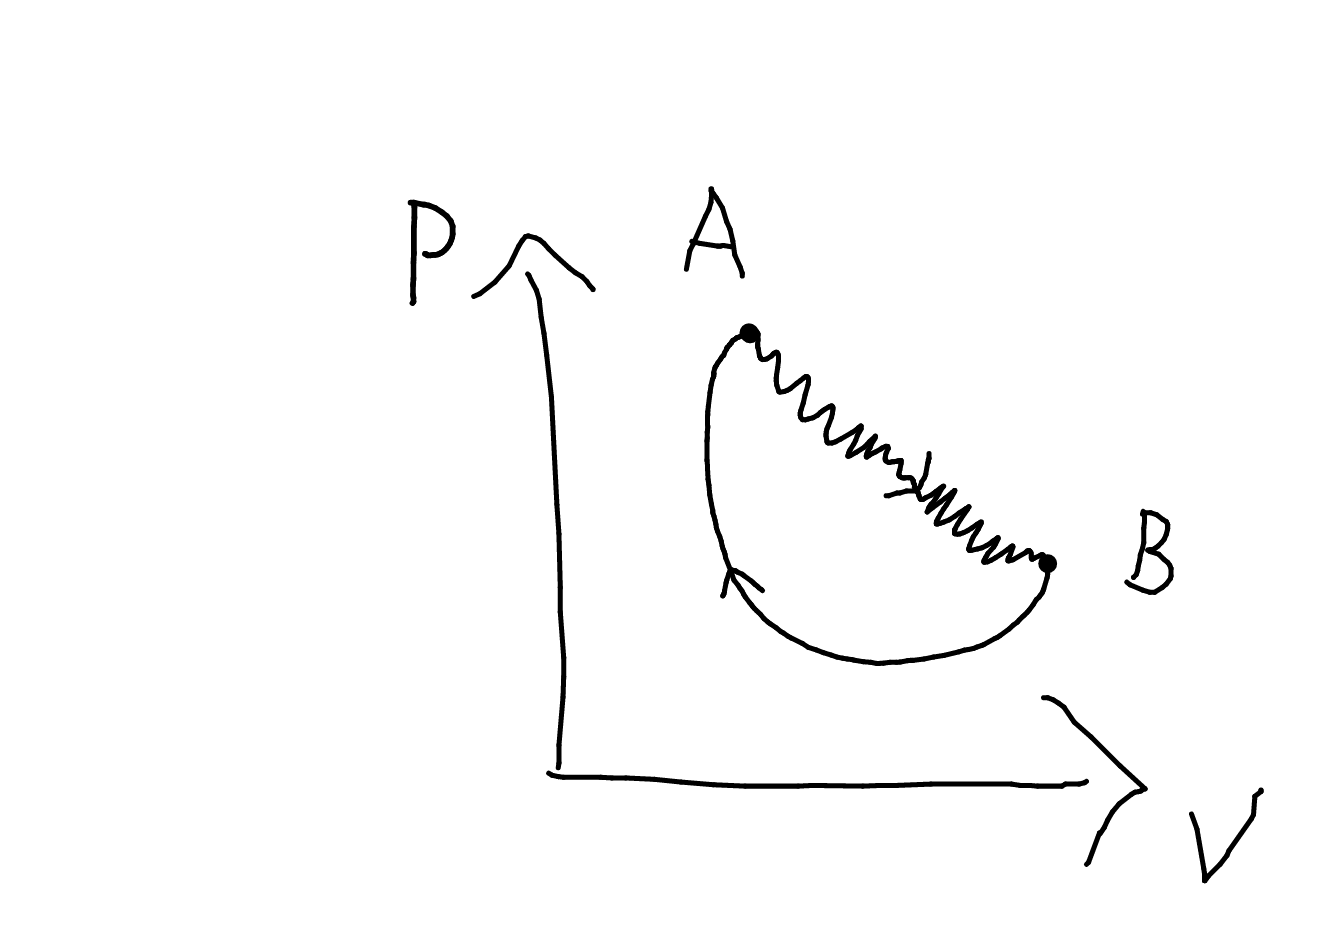
\includegraphics[width=0.5\textwidth]{TrasfAperta.png}
    \label{TrasformazioneAperta}
\end{figure}
Possiamo quindi applicare la disuguaglianza integrale nel caso generale esplicitando l'integrale:
\begin{equation}
\begin{split}
    \oint\frac{\delta Q}{T}&=\int_A^B\frac{\delta Q_{irr}}{T_S}+\int_B^A\frac{\delta Q_{rev}}{T}=\\
    &=\int_A^B\frac{\delta Q_{irr}}{T_S}+\int_B^A\dif S=\int_A^B\frac{\delta Q_{irr}}{T_S}-\int_A^B\dif S=\\
    &=\int_A^B\frac{\delta Q_{irr}}{T_S}-\left[S(B)-S(A)\right]\leq 0
\end{split}
\end{equation}
Otteniamo quindi:
\[\boxed{\int_A^B\frac{\delta Q_{irr}}{T_S}\leq S(B)-S(A)}\]
Che rappresenta la forma più generale della disuguaglianza di Clausius e rappresenta una formulazione matematica del secondo principio della termodinamica, includendo un importante risultato matematico (l'esistenza della funzione di stato \textbf{entropia}) e uno fisico (la disuguaglianza, ottenuta dall'enunciato di Kelvin).
\end{prop}
\note Nel caso di n sorgenti vale invece:
\[\sum_i\frac{Q_i}{T_i}\leq S(B)-S(A)\]
Inoltre, essendo l'entropia una funzione di stato, è possibile calcolarla direttamente solo per trasformazioni reversibili, mentre per quelle \textbf{irreversibili} si può calcolare \textit{combinando le variazioni di entropia di altre due trasformazioni reversibili}.
\subsection{La Variazione di Entropia di Alcune Trasformazioni}
\paragraph{Solidi e Liquidi}
Durante le trasformazioni di fase il calore scambiato con una certa massa di sostanza vale:
\[Q=\pm m\lambda\]
Calcoliamo l'integrale di Clausius:
\begin{equation}
    \Delta S=\int \frac{\dif Q_{rev}}{T_0}=\frac{Q}{T_0}=\pm\frac{m\lambda}{T_0}
\end{equation}
Quando invece i solidi e liquidi passano da una temperatura all'altra:
\[\Delta S=\int_A^B\frac{\delta Q}{T}=mc\int_A^B\frac{\dif T}{T}=mc\ln\frac{T_B}{T_A}\]
\paragraph{Trasformazioni Reversibili dei Gas}
Per ogni trasformazioni reversibile possiamo applicare il seguente ragionamento:
\begin{equation}
\begin{split}
    \dif S&=\frac{\delta Q_{rev}}{T}=n\overline{c}_V\frac{\dif T}{T}+\frac{1}{T}p\dif V=\\
    &=n\overline{c}_V\frac{\dif T}{T}+\frac{1}{T}\frac{nRT}{V}\dif V=\\
    &=n\overline{c}_V\frac{\dif T}{T}+\frac{nR}{V}\dif V=n\overline{c}_V\frac{\dif T}{T}+nR\frac{\dif V}{V}=\\
    &=n\overline{c}_V\left[\frac{\dif T}{T}+\frac{\overline{c}_p-\overline{c}_V}{\overline{c}_V}\frac{\dif V}{V}\right]=\\
    &=n\overline{c}_V\left[\frac{\dif T}{T}+(\gamma-1)\frac{\dif V}{V}\right]
\end{split}
\end{equation}
Calcoliamo ora l'integrale di Clausius:
\begin{equation}
\begin{split}
    \Delta S&=\int_A^B\dif S=\int_A^Bn\overline{c}_V\left[\frac{\dif T}{T}+(\gamma-1)\frac{\dif V}{V}\right]=\\
    &=n\overline{c}_V\int_A^B\left[\frac{\dif T}{T}+(\gamma-1)\frac{\dif V}{V}\right]=\\
    &=n\overline{c}_V\left[\ln\frac{T_B}{T_A}+(\gamma-1)\ln\frac{V_B}{B_A}\right]=\\
    &=n\overline{c}_V\left[\ln\frac{T_B}{T_A}+\left(\ln\frac{V_B}{B_A}\right)^{\gamma-1}\right]=\\
    &=n\overline{c}_V\ln\left[\frac{T_B}{T_A}\left(\frac{V_B}{B_A}\right)^{\gamma-1}\right]=\\
    &=n\overline{c}_V\ln\left[\frac{T_BV_B^{\gamma-1}}{T_AV_A^{\gamma-1}}\right]
\end{split}
\end{equation}
Possiamo quindi esprimere in tre modi la variazione di entropia:
\[\Delta S=n\overline{c}_V\ln\left[\frac{T_BV_B^{\gamma-1}}{T_AV_A^{\gamma-1}}\right]=n\overline{c}_V\ln\left[\frac{p_BV_B^{\gamma}}{p_AV_A^{\gamma}}\right]=n\overline{c}_V\ln\left[\frac{T_A^{\gamma}T_B^{\gamma}}{p_A^{\gamma-1}p_B^{\gamma-1}}\right]\]
Esaminiamo ora singolarmente le maggiori trasformazioni reversibili.\\
L'\textbf{adiabatica} è la più semplice, in quanto è caratterizzata da $pV^{\gamma}=cost$, quindi otteniamo:
\[\Delta S=n\overline{c}_V\ln\left[\frac{p_BV_B^{\gamma}}{p_AV_A^{\gamma}}\right]=n\overline{c}_V\ln(1)=0\]
Ossia una trasformazione adiabatica è \textbf{isoentropica}, non cambia mai il proprio valore di Entropia.
Per quanto riguarda l'\textbf{isocora}:
\[\Delta S=n\overline{c}_V\ln\left[\frac{T_BV_B^{\gamma-1}}{T_AV_A^{\gamma-1}}\right]=n\overline{c}_V\ln\frac{T_B}{T_A}=n\overline{c}_V\ln\frac{p_B}{p_A}\]
L'\textbf{isobara}:
\[\Delta S=n\overline{c}_V\ln\left[\frac{p_BV_B^{\gamma}}{p_AV_A^{\gamma}}\right]=n\overline{c}_V\gamma\ln\frac{V_B}{V_A}=n\overline{c}_V(\frac{\overline{c}_p}{\overline{c}_V})\ln\frac{V_B}{V_A}=n\overline{c}_p\ln\frac{V_B}{V_A}=n\overline{c}_p\ln\frac{T_B}{T_A}\]
E infine l'\textbf{isoterma}:
\[\Delta S=n\overline{c}_V\ln\left[\frac{T_BV_B^{\gamma-1}}{T_AV_A^{\gamma-1}}\right]=n\overline{c}_V(\gamma-1)\ln\frac{V_B}{V_A}=n\overline{c}_V(
\frac{\overline{c}_p-\overline{c}_V}{\overline{c}_V})\ln\frac{V_B}{V_A}=n(\overline{c}_p-\overline{c}_V)\ln\frac{V_B}{V_A}=nR\ln\frac{V_B}{V_A}=nR\ln\frac{p_A}{p_B}\]
\paragraph{Espansione Libera}
Studiamo ora il caso dell'Espansione Libera di un gas come nel Secondo Esperimento di Joule. Siccome l'entropia è una funzione di stato possiamo applicare il risultato ottenuto anche ad una trasformazione irreversibile (come è tal caso) e otteniamo:
\begin{equation}
\Delta S=n\overline{c}_V\ln\left[\frac{T_fV_f^{\gamma-1}}{T_iV_i^{\gamma-1}}\right]=n\overline{c}_V\ln\frac{V_f^{\gamma-1}}{V_i^{\gamma-1}}=nR\ln\frac{V_f}{V_i}=nR\ln\frac{V_B+V_A}{V_A}>0
\end{equation}
Notiamo che la variazione di entropia è positiva, come ci si aspettava. 
\paragraph{Equilibrio Termico di due Corpi}
Dati due corpi a temperatura $T_A$ e $T_B$ rispettivamente, il calore che si scambiano è:
\[\delta Q_A=m_Ac_A\dif T\quad\delta Q_B=m_Bc_B\dif T\]
Calcoliamo l'integrale di Clausius tra lo stato iniziale e quello di equilibrio:
\[\Delta S=\Delta S_A+\Delta S_B=m_Ac_A\ln\frac{T_e}{T_A}+m_Bc_B\ln\frac{T_e}{T_B}\]
Si può dimostrare che in generale questa quantità è positiva utilizzando le proprietà dei logaritmi, considerando il caso in cui i corpi abbiano uguale massa e stesso calore specifico:
\begin{equation}
\begin{split}
    \Delta S&=mc\ln\left[\frac{(T_A+T_B)^2}{T_AT_B}\right]=\\
    &=2mc\ln\left[\frac{T_A+T_B}{\sqrt{T_AT_B}}\right]>0
\end{split}
\end{equation}
L'argomento è maggiore di 1 in quanto si può dimostrare che la media aritmetica è maggiore della media geometrica degli stessi valori. 

\paragraph{Tabella delle Trasformazioni Reversibili}
\begin{center}
\scalebox{1.5}{
\begin{tabular}{|c|c|c|c|c|}
    \hline
    \textbf{Trasformazione} & \textbf{Q} & \textbf{L} & \textbf{$\Delta U$} & \textbf{$\Delta S$}  \\
    \hline
    Isobara & $n\overline{c}_p\Delta T$ & $p_A(V_B-V_A)$ & $n\c_V\Delta T$ & $n\c_p\ln\frac{T_B}{T_A}$ \\
    \hline
    Isocora & $n\c_V\Delta T$ & 0 & $n\c_V\Delta$ & $n\c_v\ln\frac{T_B}{T_A}$\\
    \hline
    Isoterma & $L$ & $nRT\ln\frac{V_B}{V_A}$ & 0 & $nR\ln\frac{V_B}{V_A}$\\
    \hline
    Abiabatica & 0 & $-n\c_V\Delta T$ & $n\c_V\Delta T$ & 0\\
    \hline
\end{tabular}}
\end{center}

\end{document}